\chapter{A tour of the interface}
\label{ch:interface}

Start MeerK40t and you are looking at a frame full of dockable panels around one
large canvas. Nothing about the arrangement is fixed: every panel can be moved,
floated, hidden and brought back, and the arrangement you leave behind is the one
you get next time. This chapter is the floor plan.

\begin{figure}[htbp]
\centering
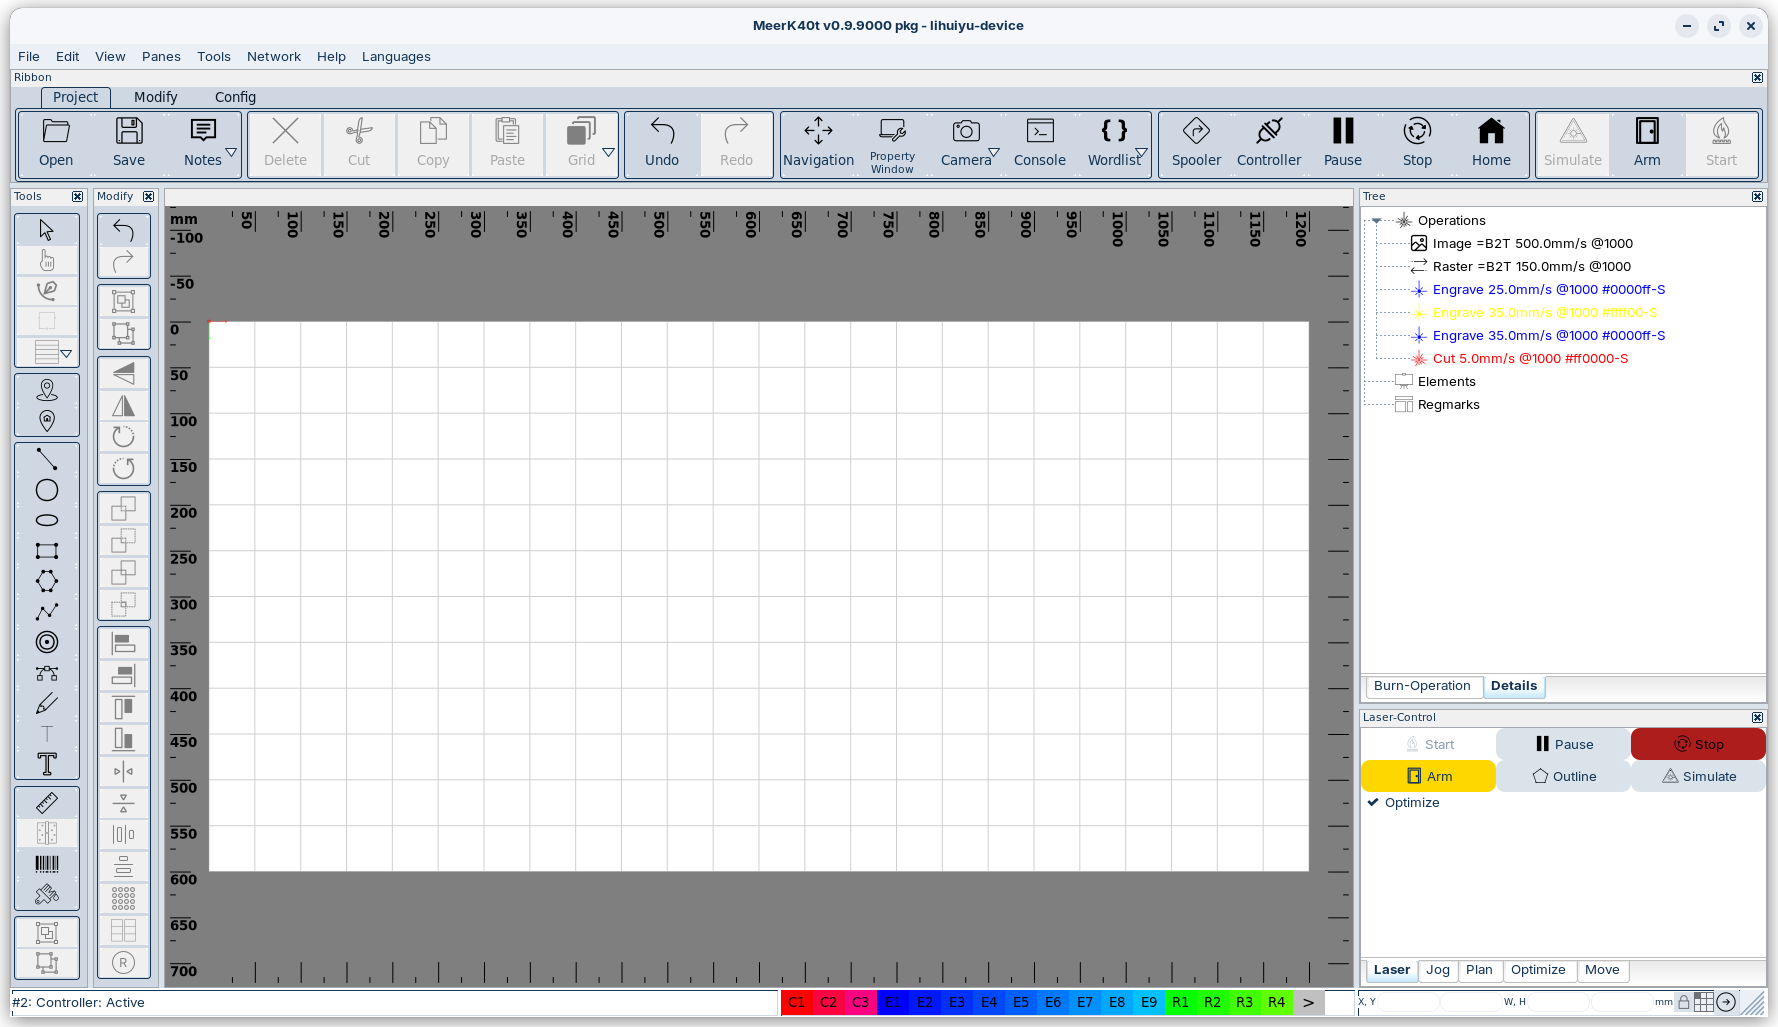
\includegraphics[width=\textwidth]{../screenshots/main.png}
\caption{A fresh MeerK40t window with the ribbon interface. Top: the ribbon
(\tabname{Project} page) with the \panel{Tools} and \panel{Modify} icon bars
docked at the left. Centre: the scene, with rulers, the bed outline, the work
origin and a laser-path preview. Right: the \panel{Tree} pane above the
\panel{Laser-Control} pane. Bottom: the status bar with its operation squares,
coordinate readouts and snap toggles.}
\label{fig:main-window}
\end{figure}

\section{The five regions}

\begin{description}[leftmargin=1.4em,style=nextline]
  \item[The menu bar] Nine menu titles at most --- \menu{File}, \menu{Edit},
        \menu{View}, \menu{Panes}, \menu{Tools}, \menu{Network}, \menu{Help} and
        (when translations are installed) \menu{Languages}. Each one is covered
        in \S\ref{sec:menus}.
  \item[The ribbon] Tool buttons arranged on pages. Three ribbon bars exist: the
        main one across the top, and two compact icon bars (\panel{Tools} and
        \panel{Modify}) usually docked down the left edge.
  \item[The scene] The canvas. This is your artwork, drawn to scale in
        millimetres, with the machine's bed as a white rectangle and the machine
        origin marked inside it.
  \item[The tree] The document outline: \emph{Operations}, \emph{Elements} and
        \emph{Regmarks}.
  \item[The status bar] Along the bottom. It holds quick-assign squares, the
        current selection's position and size, and the snap toggles.
\end{description}

\section{The scene}

Everything you draw or import appears in the scene. Three cues tell you where you
are:

\begin{itemize}
  \item \textbf{The bed rectangle} is the physical working area of your machine,
        drawn from the device's bed size setting. If your artwork is outside it,
        the job will not fit --- better to discover that here than at the machine.
  \item \textbf{The origin indicator} marks the zero point the job is measured
        from. \menu{View>Scene Appearance>Hide Origin-Indicator} turns it off.
  \item \textbf{The rulers} run along the top and left edges in the current unit
        (millimetres by default, changeable in
        \menu{Edit>Settings>Preferences}, \tabname{General}, units panel).
\end{itemize}

\noindent The grey area outside the bed is legal to draw on but will not be cut
unless you move the artwork or the job origin (Chapter~\ref{ch:where}).

\subsection*{Moving around}

\begin{center}\small
\begin{tabular}{@{}L{4.4cm}L{9.8cm}@{}}
\toprule
\textbf{Input} & \textbf{Effect} \\
\midrule
Mouse wheel & Zoom in/out around the pointer \\
\key{Shift}+wheel, or wheel left/right & Pan horizontally \\
Wheel + \key{Ctrl} & Toggle the other of zoom/pan (so \key{Ctrl}+wheel pans
vertically by default) \\
Right-drag + \key{Alt} & Drag-zoom \\
Middle-drag + \key{Ctrl} & Drag-zoom \\
Right-drag + \key{Ctrl} & Drag-pan \\
Left-drag on empty space & Rubber-band select: drag right to enclose, drag left
to touch. \key{Shift} adds to the selection, \key{Ctrl} inverts it \\
Left-drag on the selection & Move the selected elements \\
Left click & Select the element under the pointer \\
Right click & Scene menu: grids, background, ``Move laser head here'', zoom
commands \\
\bottomrule
\end{tabular}
\end{center}

\noindent Two preferences change the wheel behaviour: \setting{mouse_wheel_pan}
(\emph{MouseWheel Pan}) makes the wheel pan instead of zoom, and
\setting{mouse_pan_invert} / \setting{mouse_zoom_invert} flip the directions.
They live in \menu{Edit>Settings>Preferences}, \tabname{GUI}.

\begin{tipbox}
A three-button mouse makes layout work much nicer: \key{Ctrl}+right-drag pans,
\key{Alt}+right-drag zooms, and the left button stays free for selecting and
dragging. Practise for a minute before you start drawing.
\end{tipbox}

\section{The tree}

The \panel{Tree} pane is the document. It has exactly three branches, always in
this order:

\begin{center}\small
\begin{tabular}{@{}L{2.8cm}L{11.5cm}@{}}
\toprule
\textbf{Branch} & \textbf{What lives there} \\
\midrule
\emph{Operations} & The recipes: what to cut, engrave, raster or dot, and with
which settings. Created by you; they hold references to elements, not the
elements themselves. \\
\emph{Elements} & The artwork: paths, rectangles, ellipses, text, images, and
groups or layers holding them. \\
\emph{Regmarks} & Registration marks: shapes used to align a job with something
already on the material, or with a camera view (Chapter~\ref{ch:where}). \\
\bottomrule
\end{tabular}
\end{center}

\noindent The tree pane is itself a notebook with two tabs: \tabname{Burn-Operation}
and \tabname{Details}. Right-clicking anything in the tree gives a context menu
specific to what you clicked --- those menus are how operations get created and
how elements get assigned, and they are the subject of
Chapters~\ref{ch:ops} and~\ref{ch:tree}. Treat the tree as the control room:
most mistakes are visible here before they reach the machine.

\section{Laser-Control and the other machine panes}

\panel{Laser-Control} is the pane you will press when the job is ready. It is a
notebook with five tabs:

\begin{center}\small
\begin{tabular}{@{}L{2.0cm}L{12.3cm}@{}}
\toprule
\textbf{Tab} & \textbf{Contents} \\
\midrule
\tabname{Laser} & \btn{Start}, \btn{Pause}/\btn{Resume}, \btn{Stop},
\btn{Arm}/\btn{Disarm}, \btn{Outline}, \btn{Simulate}, the \btn{Optimize}
checkbox, the \btn{Override} checkbox with power and speed sliders, and the job
progress readout. \\
\tabname{Jog} & Manual movement of the head. \\
\tabname{Plan} & The current plan: its stages, status and contents; buttons
\btn{Update}, \btn{Export}, \btn{Spool}, checkbox \btn{Hold}. \\
\tabname{Optimize} & Recalculation controls and the optimisation settings
(Chapter~\ref{ch:order}). \\
\tabname{Move} & Position readout and move-to commands. \\
\bottomrule
\end{tabular}
\end{center}

\noindent Other panes worth knowing on day one:

\begin{center}\small
\begin{tabular}{@{}L{3.2cm}L{11.1cm}@{}}
\toprule
\textbf{Pane} & \textbf{Purpose} \\
\midrule
\panel{Console} & The command interface (Chapter~\ref{ch:console}). Open it with
the \btn{Console} button in the ribbon (or \menu{Panes>Console}) and keep it
open; it reports what the program is actually doing. \\
\panel{Position} & Numeric position and size of the selection. \\
\panel{Snap-Options} & \btn{Snap to Grid}, \btn{Snap to Element} and related
toggles. \\
\panel{Magnet-Options} & Constraint helpers for dragging. \\
\panel{Operations} & Coloured squares, one per operation, for assigning the
selection with one click (Chapter~\ref{ch:ops}). \\
\panel{Jog}, \panel{Move}, \panel{Drag}, \panel{Pulse} & Movement and
positioning controls for the machine. \\
\panel{Spooler} & The job queue and the history of completed jobs
(Chapter~\ref{ch:order}). \\
\panel{Devices} & The list of configured machines. \\
\panel{Notes} & Free-text notes attached to the current file. \\
\panel{Wordlist} & Text lists used for serial-number style production work. \\
\panel{Tasks} & Background tasks and threads, for troubleshooting. \\
\bottomrule
\end{tabular}
\end{center}

\section{Panes: hiding, showing and resetting}
\label{sec:panes}

Every pane appears as a check item in the \menu{Panes} menu, sorted into
submenus --- \emph{Laser}, \emph{Navigation}, \emph{Editing}, \emph{Tools},
\emph{Help} and \emph{Debug}. Click an item to show or hide that pane. Three more
commands sit at the bottom of the same menu:

\begin{itemize}
  \item \btn{Lock Panes} --- freeze the layout so a stray drag cannot rearrange
        anything.
  \item \btn{Reset Panes} --- restore the default layout.
  \item \emph{Long UI descriptions (ribbon + context menus)} --- whether hovering
        a button or menu item shows the long explanation or just the short one.
\end{itemize}

\noindent \menu{View>GUI Appearance>Show/Hide UI-Panels} (or \key{Ctrl+U}) hides
every visible pane at once, leaving only the scene --- convenient on a small
screen. Press it again to get everything back.

\begin{tipbox}
The console can do all of this too, which is handy for scripting a familiar
layout: \cmd{pane show console}, \cmd{pane hide tree}, \cmd{pane float jog},
\cmd{pane reset}, \cmd{pane lock}, \cmd{pane save mysetup} and
\cmd{pane load mysetup}.
\end{tipbox}

\section{The menus}
\label{sec:menus}

The menu bar is stable; the ribbon changes. Both reach the same commands. The
important entries:

\begin{center}\small
\begin{tabular}{@{}L{2.1cm}L{13.2cm}@{}}
\toprule
\textbf{Menu} & \textbf{What you will use it for} \\
\midrule
\menu{File} &
\btn{New} (\key{Ctrl+N}) clears operations, elements and notes.
\btn{Open Project} (\key{Ctrl+O}) loads a project.
\btn{Import File} merges artwork into the current project.
\btn{Save} / \btn{Save As} write the project.
Holding \key{Shift} while loading asks where the imported elements should be
placed. A \emph{Recent} submenu lists recent files, with \btn{Clear project on
load} and \btn{Clear Recent}. \\
\menu{Edit} &
\btn{Undo} / \btn{Redo} (with a submenu of undo steps),
\btn{Cut} / \btn{Copy} / \btn{Paste} / \btn{Paste from system},
\btn{Select all} (\key{Ctrl+A}), \btn{Select None},
\btn{Invert selection} (\key{Ctrl+I}), \btn{Select all non-assigned},
\btn{Delete}, \btn{Properties}. Further down: \btn{Device-Manager},
\btn{Device-Configuration}, and the \emph{Settings} submenu with
\btn{Wordlist-Editor}, \btn{CSV Batch Run}, \btn{Camera Calibration},
\btn{Font-Manager}, \btn{Key-Bindings} and \btn{Preferences} (\key{Ctrl+,}). \\
\menu{View} &
Zoom commands (\key{Ctrl+-}, \key{Ctrl++}, \key{Ctrl+B} zoom to bed,
\key{Ctrl+Shift+B} zoom to selection), \btn{Show Variables}, and three submenus:
\emph{GUI Appearance}, \emph{Scene Appearance} (hide grid, background, guides,
regmarks, laser path, reticle; invert; flip XY) and \emph{Render-Options}
(ignore shapes, text or images when drawing and when burning). \\
\menu{Panes} & Pane visibility, locking and resetting --- see \S\ref{sec:panes}. \\
\menu{Tools} & Every separate window: \panel{Properties}, \panel{Console},
\btn{Preferences}, \btn{About}, \btn{Keymap}, \btn{Wordlist},
\btn{CSV Batch Run}, \btn{Material Library}, \btn{Navigation}, \btn{Notes},
\btn{Auto-Exec}, \btn{Spooler}, \btn{Tasks}, \btn{Simulation},
\btn{Execute Job}, \btn{Device Manager}, \btn{Camera Calibration},
\btn{Font-Manager}, \btn{Image Splitter}, \btn{Operation Info},
\btn{Place Template}, \btn{Parameter-Test} and the per-device windows
(\btn{Controller}, \btn{Configuration}, \btn{Rotary}, \btn{Cylinder}, and so on),
plus \btn{Reset Windows}. \\
\menu{Network} & Start and stop the Web, Telnet, Ruida and GRBL servers ---
remote control (Chapter~\ref{ch:remote}). \\
\menu{Help} & \btn{Help} (\key{F1}) and \btn{Online Reference} (\key{F11}) open
the wiki page for whatever is under the mouse; \btn{Beginners' Help},
\btn{Github}, \btn{Releases}, \btn{Facebook}, \btn{Discord},
\btn{Makers Forum}, \btn{Feature request/feedback}, \btn{Check for Updates},
\btn{Tips \&\& Tricks} and \btn{About MeerK40t}. \\
\menu{Languages} & Switch interface language. Takes effect after a restart. \\
\bottomrule
\end{tabular}
\end{center}

\begin{behindbox}[Context-sensitive help is worth knowing]
\key{F1} does not open one fixed page. MeerK40t looks at the widget under your
mouse, reads its help tag, and opens the wiki page for that feature at
\file{https://github.com/meerk40t/meerk40t/wiki/}. Hover over the \btn{Kerf}
field, press \key{F1}, and you get the kerf page. It is the fastest way to
answer ``what is this box for?'' without leaving the program.
\end{behindbox}

\section{The ribbon}

The ribbon is the toolbar, and it comes in three pieces:

\begin{itemize}
  \item the main \panel{Ribbon} across the top, with three pages ---
        \tabname{Project}, \tabname{Modify} and \tabname{Config};
  \item two vertical icon bars on the left, \panel{Tools} (drawing and selection
        tools) and \panel{Modify} (transform and alignment tools).
\end{itemize}

\noindent Ribbon buttons from your device plugins also appear here ---
\btn{Pause}, \btn{Stop} and \btn{Home} for GRBL, \btn{Red Dot} for diode
machines, \btn{Galvo Light} and \btn{Center} for galvo, \btn{Focus Z} for Ruida,
and so on. Depending on what is configured, some pages will look busier than
Figure~\ref{fig:main-window} suggests.

\begin{tipbox}
Do not like the defaults? \menu{Edit>Settings>Preferences}, tab
\tabname{Ribbon}, lets you add, remove and reorder pages, panels and buttons;
\btn{Reset to Default} puts everything back. You can also switch pages from the
console with \cmd{page project}, \cmd{page modify} or \cmd{page config}.
\end{tipbox}

\section{The status bar}

Left to right, the status bar gives you: a message area (it also shows the
description of whatever menu item you are hovering), then a row of
\emph{operation squares}, then the selection readout and snap toggles.

The operation squares are the fastest way to classify artwork. Each square is one
operation, coloured with that operation's colour. Click a square with elements
selected and they are assigned to that operation. In
Figure~\ref{fig:main-window} you can see them labelled \emph{C1}, \emph{C2},
\emph{C3}, \emph{E1}--\emph{E9} and \emph{R1}--\emph{R4}: cuts, engravings and
rasters. Chapter~\ref{ch:ops} explains the colour rules in full.

\section{Windows that are not panes}

Some features open as separate windows rather than docks: \btn{Preferences},
\btn{Keymap}, \btn{Wordlist}, \btn{Material Library}, \btn{Parameter-Test},
\btn{Simulation}, \btn{Execute Job}, \btn{Device Manager}, \btn{Camera
Calibration}, \btn{Image Splitter}, \btn{Operation Info}, \btn{Place Template}
and \btn{About}. They are all listed in the \menu{Tools} menu, and
\btn{Reset Windows} forgets their stored positions if one ends up off-screen.

\section{The simplified interface}

If the full window feels like an aircraft cockpit, launch with \cmd{-w} (or
\cmd{--simpleui}) for a stripped-down version: a window with four pages ---
\tabname{Project} (load a project and see whether it is ready to burn),
\tabname{Laser}, \tabname{Jog+Move} and \tabname{Console}. The project page
summarises the current file: how many elements, how many burn operations, and
either ``Ready to burn.'', ``Unassigned elements!'' or ``Unburnable elements!''.
That single line is a good habit even in the full interface: it tells you the
job is complete before the machine does.

\begin{tryit}{Make the window yours}
\begin{enumerate}[label=\arabic*.,leftmargin=1.4em]
  \item Open the \panel{Console} pane (its button is in the ribbon under
        \menu{Panes}, and you can bind \key{F12} to \cmd{window open Console} in
        the Keymap window if you want it) and the \panel{Position} pane
        (\menu{Panes>Editing>Position}).
  \item Drag the \panel{Console} pane by its caption to the bottom edge until it
        docks there. Notice the docking hints.
  \item Press \key{Ctrl+U} twice: everything disappears, then comes back.
  \item Right-click the \panel{Tree} pane caption and float it, then dock it back
        on the right.
  \item Tick \btn{Lock Panes} in the \menu{Panes} menu, try to drag a pane, and
        confirm it will not move. Untick it again.
  \item In the console, type \cmd{pane reset}. The layout returns to the default.
  \item Close the program and reopen it. Whatever layout you had at closing is
        restored.
\end{enumerate}
\end{tryit}

\noindent Keyboard shortcuts and mouse behaviour are collected in
Appendix~\ref{app:shortcuts}; you do not need to memorise them now. The four
worth learning today are \key{Ctrl+U} (show and hide the panes), \key{Ctrl+B}
(zoom to bed), \key{Ctrl+S} (save) and \key{Home} (send the head home). None of
them is more than a menu click away, and all of them can be changed in the
Keymap window.
